\documentclass[11pt]{article}
\usepackage{amsmath,amssymb,enumitem,algorithm,algpseudocode}
\usepackage[UTF8]{ctex}
\usepackage[braket]{qcircuit}
\usepackage{tikz}
\usepackage{xcolor}
\definecolor{mygreen}{HTML}{E7F5E8}
\definecolor{myblue}{HTML}{E8F0FF}

\parindent=22pt
\parskip=3pt
\oddsidemargin 18pt \evensidemargin 0pt
\leftmargin 1.5in
\marginparwidth 1in \marginparsep 0pt \headsep 0pt \topskip 20pt
\textheight 225mm \textwidth 148mm
\renewcommand{\baselinestretch}{1.15}

\begin{document}
\title{{\bf 理论作业三 \quad 量子纠错}}
\author{姓名 \quad 学号}
\date{\today}
\maketitle

\begin{tabular*}{13cm}{r}
\hline
\end{tabular*}

\vskip 0.3 in

{\bf 1.} 写出 9 量子比特 Shor 编码的稳定子,并证明其稳定 $\{\ket{0_L}, \ket{1_L}\}$ 张成的向量空间,其中
\begin{align*}
\ket{0_L} &= \frac{(\ket{000}+\ket{111})(\ket{000}+\ket{111})(\ket{000}+\ket{111})}{2\sqrt{2}} \\
\ket{1_L} &= \frac{(\ket{000}-\ket{111})(\ket{000}-\ket{111})(\ket{000}-\ket{111})}{2\sqrt{2}}
\end{align*}

\vskip 0.3 in

{\bf 2.} 证明操作 $\bar{Z}=X_1X_2X_3X_4X_5X_6X_7X_8X_9$ 和 $\bar{X}=Z_1Z_2Z_3Z_4Z_5Z_6Z_7Z_8Z_9$ 可以充当 Shor 编码中逻辑量子比特上的逻辑 $Z$ 操作和逻辑 $X$ 操作。(提示:推导 $\bar{Z}$ 和 $\bar{X}$ 作用在 $\ket{0_L}$ 和 $\ket{1_L}$ 上的形式)

\vskip 0.3 in

{\bf 3.} 下图展示了一个二维网格上码距为 3 的表面码。其中,空心圆点表示数据量子比特,实心圆点表示辅助量子比特,每个辅助量子比特对其相邻的数据量子比特执行征状测量。写出该纠错码的稳定子,并推导逻辑态 $\ket{0_L}$ 和 $\ket{1_L}$ 的形式。
\begin{center}
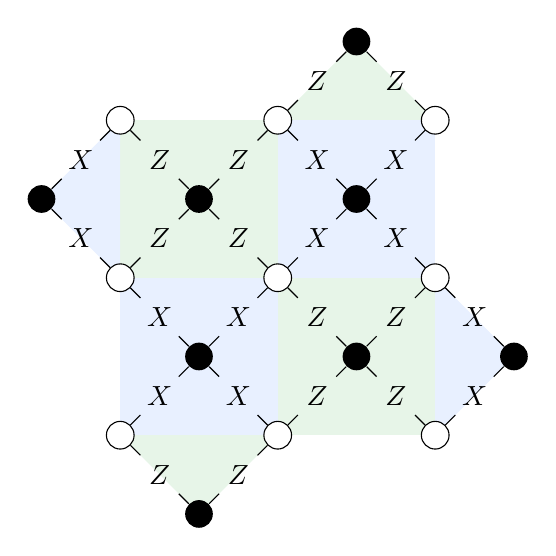
\begin{tikzpicture}
    \fill[mygreen] (0, 2.0) -- (1.0, 3.0) -- (2.0, 2.0) -- cycle;
    \fill[mygreen] (-2.0, 2.0) rectangle (0, 0);
    \fill[mygreen] (0, 0) rectangle (2.0, -2.0);
    \fill[mygreen] (0, -2.0) -- (-1.0, -3.0) -- (-2.0, -2.0) -- cycle;
    \fill[myblue] (-2.0, 0) -- (-3.0, 1.0) -- (-2.0, 2.0) -- cycle;
    \fill[myblue] (0, 2.0) rectangle (2.0, 0);
    \fill[myblue] (0, -2.0) rectangle (-2.0, 0);
    \fill[myblue] (2.0, 0) -- (3.0, -1.0) -- (2.0, -2.0) -- cycle;
    \node[circle, minimum size=10pt, draw=black, fill=white] (1) at (-2.0, 2.0) {};
    \node[circle, minimum size=10pt, draw=black, fill=white] (2) at (0, 2.0) {};
    \node[circle, minimum size=10pt, draw=black, fill=white] (3) at (2.0, 2.0) {};
    \node[circle, minimum size=10pt, draw=black, fill=white] (4) at (-2.0, 0) {};
    \node[circle, minimum size=10pt, draw=black, fill=white] (5) at (0, 0) {};
    \node[circle, minimum size=10pt, draw=black, fill=white] (6) at (2.0, 0) {};
    \node[circle, minimum size=10pt, draw=black, fill=white] (7) at (-2.0, -2.0) {};
    \node[circle, minimum size=10pt, draw=black, fill=white] (8) at (0, -2.0) {};
    \node[circle, minimum size=10pt, draw=black, fill=white] (9) at (2.0, -2.0) {};
    \node[circle, minimum size=10pt, fill=black] (10) at (1.0, 3.0) {};
    \node[circle, minimum size=10pt, fill=black] (11) at (-1.0, 1.0) {};
    \node[circle, minimum size=10pt, fill=black] (12) at (1.0, -1.0) {};
    \node[circle, minimum size=10pt, fill=black] (13) at (-1.0, -3.0) {};
    \node[circle, minimum size=10pt, fill=black] (14) at (-3.0, 1.0) {};
    \node[circle, minimum size=10pt, fill=black] (15) at (1.0, 1.0) {};
    \node[circle, minimum size=10pt, fill=black] (16) at (-1.0, -1.0) {};
    \node[circle, minimum size=10pt, fill=black] (17) at (3.0, -1.0) {};
    \node (18) at (0.5, 2.5) {$Z$};
    \draw (10) -- (18) -- (2) node[midway] {};
    \node (19) at (1.5, 2.5) {$Z$};
    \draw (10) -- (19) -- (3) node[midway] {};
    \node (20) at (-1.5, 1.5) {$Z$};
    \draw (11) -- (20) -- (1) node[midway] {};
    \node (21) at (-0.5, 1.5) {$Z$};
    \draw (11) -- (21) -- (2) node[midway] {};
    \node (22) at (-1.5, 0.5) {$Z$};
    \draw (11) -- (22) -- (4) node[midway] {};
    \node (23) at (-0.5, 0.5) {$Z$};
    \draw (11) -- (23) -- (5) node[midway] {};
    \node (24) at (0.5, -0.5) {$Z$};
    \draw (12) -- (24) -- (5) node[midway] {};
    \node (25) at (1.5, -0.5) {$Z$};
    \draw (12) -- (25) -- (6) node[midway] {};
    \node (26) at (0.5, -1.5) {$Z$};
    \draw (12) -- (26) -- (8) node[midway] {};
    \node (27) at (1.5, -1.5) {$Z$};
    \draw (12) -- (27) -- (9) node[midway] {};
    \node (28) at (-1.5, -2.5) {$Z$};
    \draw (13) -- (28) -- (7) node[midway] {};
    \node (29) at (-0.5, -2.5) {$Z$};
    \draw (13) -- (29) -- (8) node[midway] {};
    \node (30) at (-2.5, 1.5) {$X$};
    \draw (14) -- (30) -- (1) node[midway] {};
    \node (31) at (-2.5, 0.5) {$X$};
    \draw (14) -- (31) -- (4) node[midway] {};
    \node (32) at (0.5, 1.5) {$X$};
    \draw (15) -- (32) -- (2) node[midway] {};
    \node (33) at (1.5, 1.5) {$X$};
    \draw (15) -- (33) -- (3) node[midway] {};
    \node (34) at (0.5, 0.5) {$X$};
    \draw (15) -- (34) -- (5) node[midway] {};
    \node (35) at (1.5, 0.5) {$X$};
    \draw (15) -- (35) -- (6) node[midway] {};
    \node (36) at (-1.5, -0.5) {$X$};
    \draw (16) -- (36) -- (4) node[midway] {};
    \node (37) at (-0.5, -0.5) {$X$};
    \draw (16) -- (37) -- (5) node[midway] {};
    \node (38) at (-1.5, -1.5) {$X$};
    \draw (16) -- (38) -- (7) node[midway] {};
    \node (39) at (-0.5, -1.5) {$X$};
    \draw (16) -- (39) -- (8) node[midway] {};
    \node (40) at (2.5, -0.5) {$X$};
    \draw (17) -- (40) -- (6) node[midway] {};
    \node (41) at (2.5, -1.5) {$X$};
    \draw (17) -- (41) -- (9) node[midway] {};
\end{tikzpicture}
\end{center}

\end{document}
